\documentclass{report}

%%%%%%%%%%%%%%%%%%%%%%%%%%%%%%%%%%
%%%%%%% AVAILABLE SECTIONS %%%%%%%
%%%%%%%%%%%%%%%%%%%%%%%%%%%%%%%%%%
% \dfn{Title}{Contents} - Definition
% \qs{Title}{Contents} - Questions
% \dfn{Title}{Contents}
% \dfn{Title}{Contents}


\input{preamble}

\title{\Huge{Some Class}\\Random Examples}
\author{\huge{Your Name}}
\date{}

\begin{document}

\maketitle
\newpage
\pdfbookmark[section]{\contentsname}{toc}
\tableofcontents
\pagebreak

\chapter{}
\section{What is a Vector?}
\dfn{4.1}{Something}
\qs{What?}{Is the set a closed set}
\nt{We will do topology in Normed Linear Space  (Mainly and occasionally)using the language of Metric Space}
\clm{Topology}{}{Topology is cool}
\ex{Open Set and Close Set}{Sets}
\thm{}{If $x\in$ open set $V$ then $\exists$ $\delta>0$ such that $B_{\delta}(x)\subset V$}
\begin{myproof}By openness of $V$, $x\in B_r(u)\subset V$
	\begin{center}
		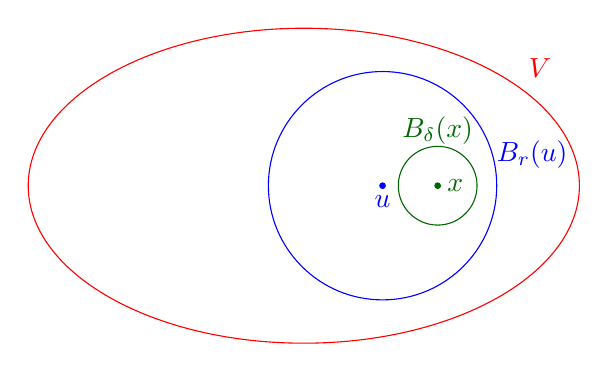
\begin{tikzpicture}
			\draw[red] (0,0) circle [x radius=3.5cm, y radius=2cm] ;
			\draw (3,1.5) node[red]{$V$};
			\draw [blue] (1,0) circle (1.45cm) ;
			\filldraw[blue] (1,0) circle (1pt) node[anchor=north]{$u$};
			\draw (2.9,0.4) node[blue]{$B_r(u)$};
			\draw [green!40!black] (1.7,0) circle (0.5cm) node [yshift=0.7cm]{$B_{\delta}(x)$} ;
			\filldraw[green!40!black] (1.7,0) circle (1pt) node[anchor=west]{$x$};
		\end{tikzpicture}
	\end{center}

	Given $x\in B_r(u)\subset V$, we want $\delta>0$ such that $x\in B_{\delta} (x)\subset B_r(u)\subset V$. Let $d=d(u,x)$. Choose $\delta $ such that $d+\delta<r$ (e.g. $\delta<\frac{r-d}{2}$)

	If $y\in B_{\delta}(x)$ we will be done by showing that $d(u,y)<r$ but $$d(u,y)\leq d(u,x)+d(x,y)<d+\delta<r$$
\end{myproof}

\cor{}{By the result of the proof, we can then show...}
\mlenma{}{}
\mprop{}{$1 + 1 = 2$.}

\section{Random}
\dfn{Normed Linear Space and Norm $\boldsymbol{\|\cdot\|}$}{}


\ex{Definition}{}
\qs{}{}
\sol{\textbf{For Property for norm-2}	\subsubsection*{When field is} We have to show\begin{align*}
		         & \sum_i(x_i+y_i)^2\leq \left(\sqrt{\sum_ix_i^2} +\sqrt{\sum_iy_i^2}\right)^2                                       \\
		\implies & \sum_i (x_i^2+2x_iy_i+y_i^2)\leq \sum_ix_i^2+2\sqrt{\left[\sum_ix_i^2\right]\left[\sum_iy_i^2\right]}+\sum_iy_i^2 \\
		\implies & \left[\sum_ix_iy_i\right]^2\leq \left[\sum_ix_i^2\right]\left[\sum_iy_i^2\right]
	\end{align*}So in other words prove $\langle x,y\rangle^2 \leq \langle x,x\rangle\langle y,y\rangle$ where
	$$\langle x,y\rangle =\sum\limits_i x_iy_i$$

	\begin{note}
    Something
	\end{note}Now the statement is just the Cauchy-Schwartz Inequality. For proof $$\langle x,y\rangle^2\leq \langle x,x\rangle\langle y,y\rangle $$ expand everything of $\langle x-\lambda y,x-\lambda y\rangle$ which is going to give a quadratic equation in variable $\lambda $ \begin{align*}
		\langle x-\lambda y,x-\lambda y\rangle & =\langle x,x-\lambda y\rangle-\lambda\langle y,x-\lambda y\rangle                                       \\
		                                       & =\langle x ,x\rangle -\lambda\langle x,y\rangle -\lambda\langle y,x\rangle +\lambda^2\langle y,y\rangle \\
		                                       & =\langle x,x\rangle -2\lambda\langle x,y\rangle+\lambda^2\langle y,y\rangle
	\end{align*}Now unless $x=\lambda y$ we have $\langle x-\lambda y,x-\lambda y\rangle>0$ Hence the quadratic equation has no root therefore the discriminant is greater than zero.

	\subsubsection*{\textbf{When field is }}Modify the definition by $$\langle x,y\rangle=\sum_i\overline{x_i}y_i$$Then we still have $\langle x,x\rangle\geq 0$}

\section{Algorithms}
\begin{algorithm}[H]
\KwIn{This is some input}
\KwOut{This is some output}
\SetAlgoLined
\SetNoFillComment
\tcc{This is a comment}
\vspace{3mm}
some code here\;
$x \leftarrow 0$\;
$y \leftarrow 0$\;
\uIf{$ x > 5$} {
    x is greater than 5 \tcp*{This is also a comment}
}
\Else {
    x is less than or equal to 5\;
}
\ForEach{y in 0..5} {
    $y \leftarrow y + 1$\;
}
\For{$y$ in $0..5$} {
    $y \leftarrow y - 1$\;
}
\While{$x > 5$} {
    $x \leftarrow x - 1$\;
}
\Return Return something here\;
\caption{what}
\end{algorithm}

\end{document}
